\documentclass[a4paper,utf8]{article}
\usepackage{graphicx}
\usepackage[heading,fancyhdr]{ctex}
\usepackage{amsmath,amssymb,geometry,ulem}
\usepackage{array,tabularx,tabulary,mhchem,xspace}
\usepackage{floatrow,subfig,multirow,bigstrut}
\usepackage{siunitx,booktabs,longtable,nameref}
\lineskiplimit=1pt
\lineskip=3pt
\geometry{
    top=25.4mm, 
    left=25mm, 
    right=25mm, 
    bottom=25mm,
    headsep=5.9mm,
}
\ctexset{
    chapter = {
        name = {实验,},
        beforeskip = {-23pt}
    }
}
\newcommand{\fgref}[1]{图~\ref{#1}\xspace}
\newcommand{\seqref}[1]{式~(\ref{#1})}
\newcommand{\expinfo}[6][无]{
    {\zihao{-3}\bfseries\songti
    实验名称:\uline{\hfill\mbox{#2}\hfill} \\[2.9mm]
    学\quad 号:\uline{\makebox[25mm]{#3}}\hfill
    姓\quad 名:\uline{\makebox[25mm]{#4}}\hfill
    班\quad 级:\uline{\makebox[25mm]{#5}} \\[2.9mm]
    合作者:\uline{\makebox[25mm]{#1}} \hfill
    桌\quad 号:\uline{\makebox[25mm]{}}\hfill\makebox[25mm+4em]{}\\[2.9mm]
    指导教师:\uline{\makebox[30mm]{#6}}\hfill\mbox{} \\[2.9mm]
    实验日期:\uline{\makebox[30mm]{}}\hfill\mbox{} \\[58.7mm]
    }
}%\expinfo[合作者]{实验名称}{学号}{姓名}{班级}{指导教师}
\newcommand{\pointingbox}{
    {\zihao{4}\bfseries\songti%
    实验考核\\[3mm]
    \extrarowheight=3mm
    \begin{tabularx}{150mm}{|X|X|X|X|X|}\hline
        \hfil 项目 \hfil  & \hfil 实验预习 \hfil & \hfil 实验过程 \hfil & \hfil 分析与讨论 \hfil & \hfil 总评 \hfil \\[3mm] \hline
        \hfil 评价 \hfil &  &  &  &  \\[3mm] \hline
    \end{tabularx}
    }
}
\newcommand{\derivative}[2]{\frac{\mathrm{d} #1}{\mathrm{d} #2}}
\newcommand{\thinking}[2]{\textbf{#1}\\
答:\begin{minipage}[t]{0.85\textwidth}
    #2
\end{minipage}}

\pagestyle{fancy}
\fancyhf{}
%\fancyhead[C]{材料科学基础实验}
%\fancyfoot[C]{\thepage}
\fancyhead[EC]{\leftmark} \fancyhead[OC]{\rightmark}
\fancyhead[EL,OR]{\thepage}
\fancypagestyle{plain}{\renewcommand{\headrulewidth}{0pt}\fancyhf{}}

\newcounter{Rownumber}
\newcommand*{\Rown}{\stepcounter{Rownumber}\theRownumber}
\newcounter{sample}
\newcommand*{\Sam}{\stepcounter{sample}\thesample}
\newcounter{Fignumber}
\newcommand*{\Fign}{\stepcounter{Fignumber}\theFignumber}

\newcommand*{\resetRown}{\setcounter{Rownumber}{0}}
\newcommand{\qrange}[3]{\qtyrange[range-phrase = \text{$\sim$},range-units =single]{#1}{#2}{#3}}
\floatsetup[table]{capposition=top}
\newcolumntype{C}{>{\hfil}X<{\hfil}}
\renewcommand{\Nameref}[1]{\textbf{\ref{#1}~\nameref{#1}}}
\newcommand{\TTR}[0]{\watt\per\m\per\K} %导入导言
\begin{document}
\begin{center}
    {\mbox{}\\[7em]\zihao{2}\bfseries\songti%
    材料科学基础实验报告}\\[34mm]
    \expinfo{磁性材料基础测量}{22301077}{张蕴东}{22高分子}{李继玲}
    {\zihao{4}\bfseries\songti
    实验考核\\[3mm]
    \extrarowheight=3mm
    \begin{tabularx}{150mm}{|X|X|X|X|X|}\hline
        \hfil 项目 \hfil  & \hfil 实验预习 \hfil & \hfil 实验过程 \hfil & \hfil 分析与讨论 \hfil & \hfil 总评 \hfil \\[3mm] \hline
        \hfil 评价 \hfil &  &  &  &  \\[3mm] \hline
    \end{tabularx}
    }
\end{center}\newpage
\part{静态磁化特性}
\section{实验目的}
    \begin{itemize}
        \item 掌握测量铁磁材料磁滞、动态磁滞回线和基本磁化曲线的原理和方法,加深对铁磁材料基本磁性参量的理解 
        \item 学习用电子积分器测量磁感应强度
        \item 学会根据磁性材料的磁性曲线确定其矫顽力、剩余磁感强度、饱和磁感强度,磁滞损耗、磁滞损耗等磁化参数
        \item 学习测量磁性材料磁导率 $\mu$ 的 一种方法,了解磁性材料的主要特性
        \item 声明:本次实验是在已经了解磁化电流不应超过 0.8 A 的前提下,已经结合了先前实验同学的经验,想尝试找到饱和磁化电流的基础下,以保证安全为首要目的,将电流缓慢试探性提高接近 1 A,事实证明,1 A 仍不能达到饱和。
    \end{itemize}
\section{实验原理}%简单描述,含必要的公式和附图;
    铁磁材料应用广泛,从常用的永久磁铁、变压器铁芯到录音、录像、计算机存储用的磁带、磁盘等都采用各种特性的铁磁材料。铁磁材料多数是铁和其他金属元素或者非金属组成的合金以及某些包含铁的氧化物(铁氧体),他们除了具有高的磁导率外,另一个重要的磁性特点就是磁滞。铁磁材料的磁滞回线和磁化曲线表征了磁性材料的基本磁化规律,反应了磁性材料的基本参数。对铁磁材料的应用和研制有重要意义。由于磁性材料的磁化过程很复杂,影响磁性材料磁化特性的因素有很多,如:掺杂、结构、温度等。在多数场合无法用解析式来定量描述 H—B 之间的关系,只能通过实验测定它。本实验中,将待测的磁性材料做成闭合环状,上面均匀地绕两组线圈。给其中一组线圈通电流 I ,使其产生强度为 H 的磁化场,这组线圈称为初级线圈。当初级线圈中的电流发生变化时,在另外一组线圈即次级线圈中,将产生感应电动势 $\varepsilon$ ,用电子积分器测出 $\varepsilon$ ,经计算可以得到 B ,根据 H—B 的对应关系可以绘出它们的曲线。
    \subsection{初始磁化曲线}
        研究磁性材料的磁化规律,通常是通过测量磁化场的磁感强度H与磁感应强度 B 的关系来进行的。磁化曲线也叫 B-H 曲线,即表示物质中的磁场强度H与所感应的磁感应强度B之间关系的曲线。铁磁材料的磁化过程非常复杂,B 和 H 的关系如图1 所示。将处在未磁化状态的磁性材料(H=0、B=0)加以磁化,当逐渐增加磁场强度 H 时,磁感强度 B 也随之增加而非线性增加,经过一段急剧增加的过程后又缓慢下来,当 H 增大到一定值 $H_s$ 后, B 增加十分缓慢或者基本不再增加,这时磁化就达到了磁饱和。到达磁饱和的 $H_s$ 和 $B_s$ 分别称为饱和磁场强度和饱和磁感应强度(对应图1-1中的a点)。从未磁化到饱和磁化,H 和 B 对应的关系曲线称为初始磁化曲线或者起始磁化曲线。如图1-1 中 Oa所示。
        \begin{figure}[!ht]
            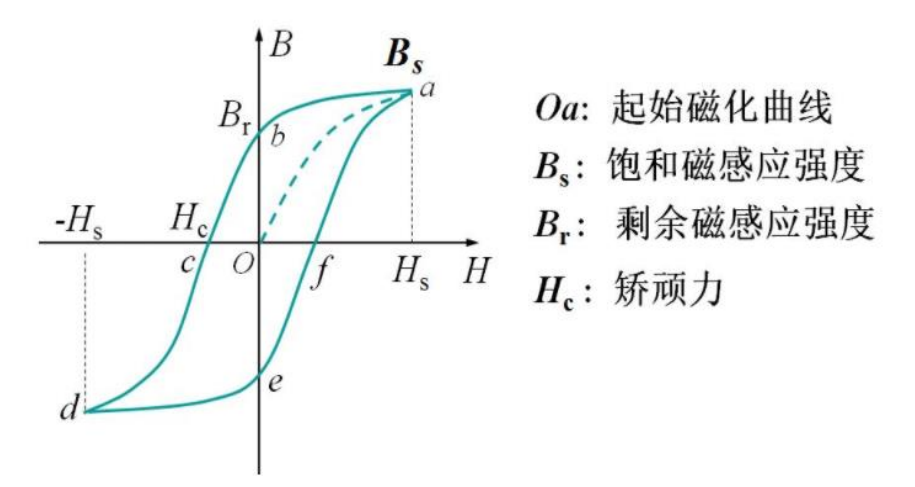
\includegraphics[width=0.6\textwidth]{fig1.png}
        \end{figure}
    \subsection{磁滞回线}
        磁性材料还有一个重要的特性,那就是磁滞。磁滞是指 B 的变化滞后于 H 的变化。如图1-1所示,当磁性材料的磁化达到饱和之后,如果使 H 单调减小,B 不沿原路沿aO返回, 而是沿一条新的路线(沿abc)下降。当 H 减小到 0,B 并不为 0,而是到达 $B_r$ ,说明此时铁磁材料中仍然保留有一定的磁性,这种现象称为磁滞效应, $B_r$ 称为剩余磁感强度,简称剩磁。要消除剩磁使 B=0 就得加一个反向的磁化场,直到反向磁化场到达 $H_c$ , B 才恢复为零。$H_c$ 被称为矫顽力。如果继续增加反向的磁化场使H继续增加,铁磁材料将被反向磁化直至达到反向饱和,此后减小磁化场 H 直至 0,再沿正方向增加 H 至饱和,曲线回到 a 点。由此得到一条 H—B 的闭合曲线,这条关于原点对称的闭合曲线,称为该材料的磁滞回线。如图1-1所示。实验表明,经过反复的磁化后,铁磁材料达到稳定的磁化状态,B-H 的量值关系形成一个稳定的闭合“磁滞回线”,通常以这条曲线来表示铁磁材料的磁化性质。
    \subsection{基本磁化曲线}
        当从初始状态(H=0, B=0)开始周期性地改变磁场强度H的幅值时,在磁场由弱变强单调增加过程中,可以得到一系列面积由小到大的稳定的磁滞回线,如图1-2所示,其中最大面积的磁滞回线称为极限磁滞回线,把图1-2中原点O和各个磁滞回线的顶点 $a_1$ , $a_2$ 等连成曲线,此曲线即为铁磁材料的基本磁化曲线。不同的铁磁材料其基本磁化曲线是不相同的。根据基本磁化曲线可以近似确定铁磁材料的磁导率 $\mu$ 。从基本磁化曲线上一点到原点 O 连线,其斜率 $μ =B/H$ 定义为这种磁化状态下的磁导率。
    \subsection{测量原理}
        测量电路如讲义图 1-3 所示,图中 A 为环状磁性材料,$N_1$、$N_2$ 分别为绕在其上的初、 次级线圈的匝数;M 为互感器;$R_0$ 是取样电阻,阻值为 1 \unit{\ohm} ;电子积分器用于测量 B,由运算放大器等构成。$K_1$ ,电流换向开关; $K_2$ ,选择测量开关;$K_3$ ,复位按钮开关;E,可调电源。\par
        磁化场 $H$ 和 磁感应强度 $B$ 表示为:
        \begin{align}
            H&=\frac{N_1 U_x}{L R_0}\label{eq:1}\\
            B&=\frac{\tau U_0}{S N_2}\label{eq:2}
        \end{align}
        实验时只要单调、缓慢地改变磁化电流 $I_0$,计算机就可以同步画出与 $H—B$ 关系相对应的 $U_x—U_0$ 曲线。$U_0$、$U_x$ 的大小可以分别从计算机所绘的曲线上求得。
\section{实验仪器}%规格及参数
    静态磁特性参数测量仪,直流电源,计算机
\section{实验过程}%简述主要过程和实验内容
    \begin{enumerate}
        \item 开启电脑,运行静态磁性测量仪应用程序,并熟悉各种操作功能;
        \item 测量初始磁化曲线:包括手动退磁和测绘曲线两个步骤
        \item 测量磁滞回线
        \item 测量基础磁化曲线
    \end{enumerate}
\section{实验数据}
    首先根据所用的仪器给出的参数记录得到下表,以通过\eqref{eq:1} 和 \eqref{eq:2} 计算 $U_x—U_0$ 曲线到 $H—B$ 曲线的比例换算关系。
    \begin{table}[!ht]
        \centering\begin{tabular}{c c|c c}\hline
             内径 & \SI{34}{\mm} & 外径 & \SI{50}{\mm} \\ \hline
             匝数 $N_1$ & \SI{34}{\mm} & 匝数 $N_2$ & \SI{50}{\mm} \\ \hline
             $\tau$ & 0.0100 &  &  \\ \hline
        \end{tabular}
    \end{table}\par
    将所得到的数据在 Origin 中处理,换算是基于 Origin 内置函数: $$A-(Max(A)+Min(A))/2 + \text{offset} $$ 的变换,先根据极值粗调,再进行细致调整(offset),以保障结果的质量。得到下图:
    \begin{figure}[!ht]
        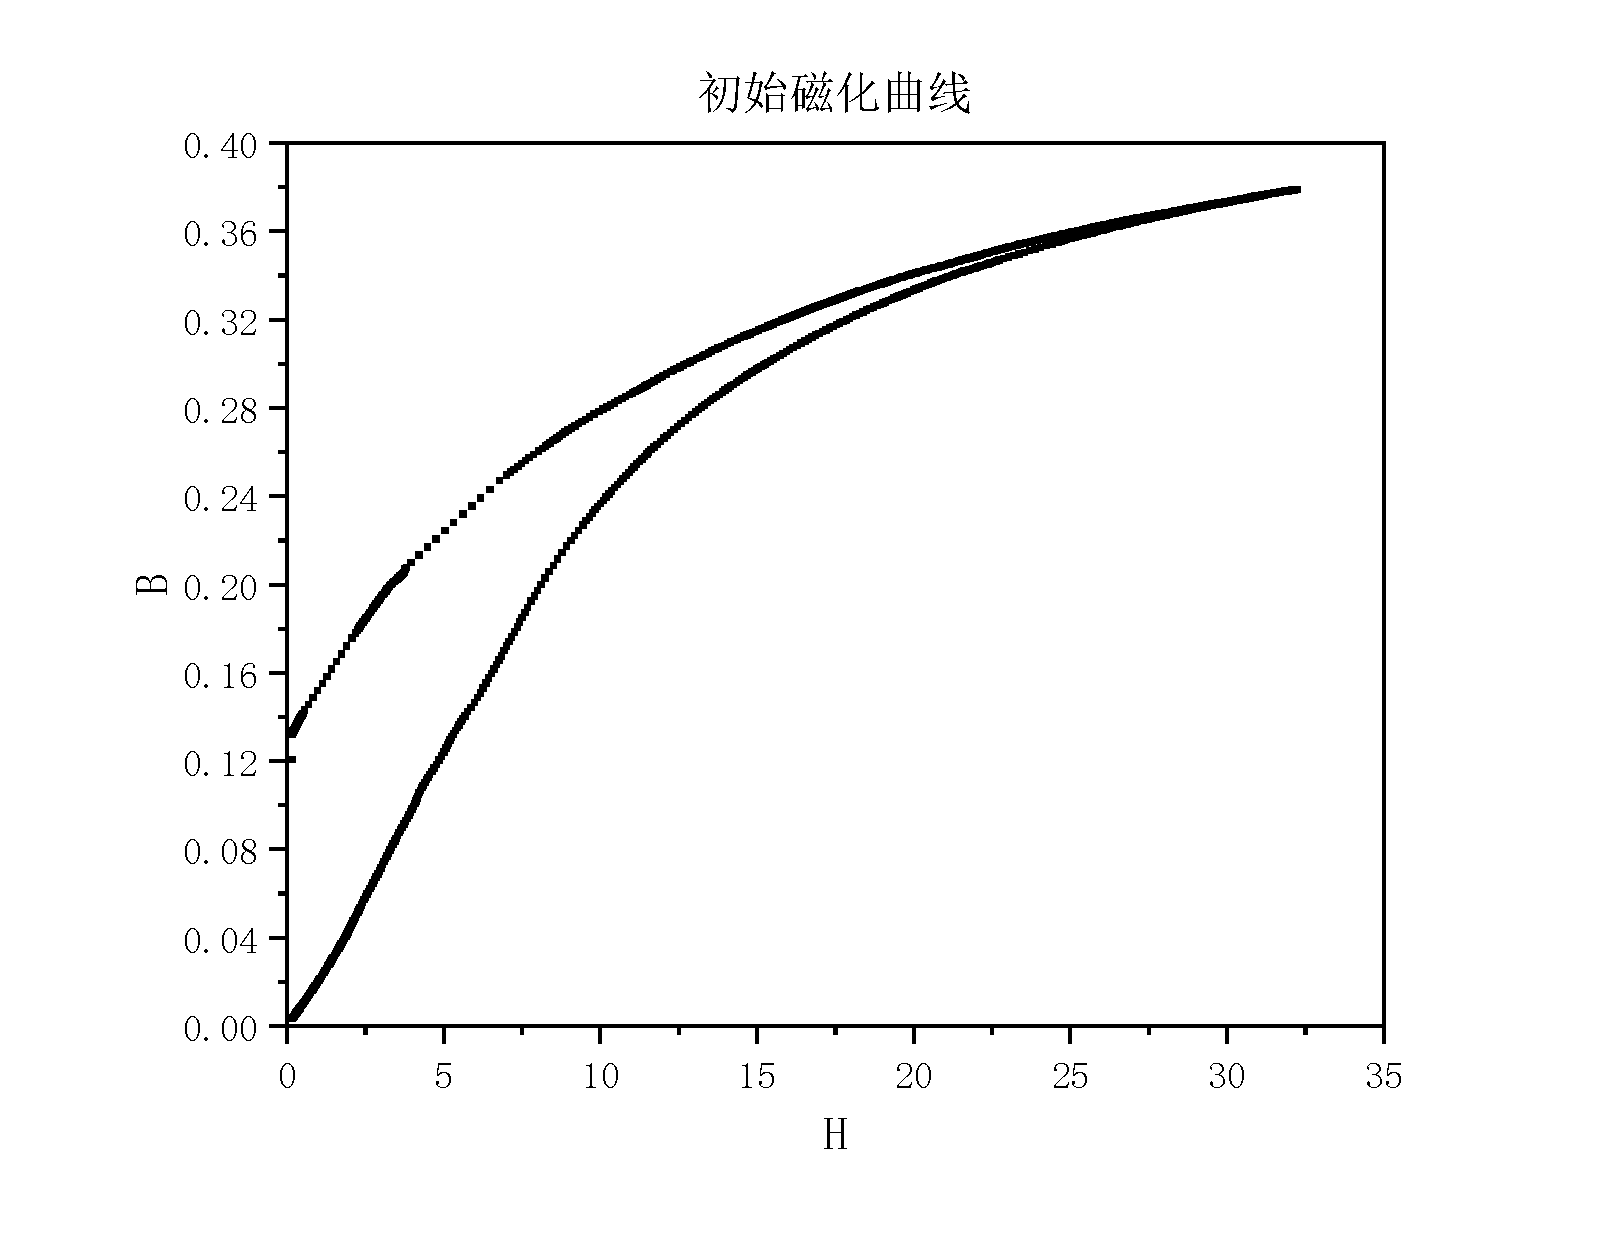
\includegraphics[width=0.6\textwidth]{fig2.pdf}
        \caption{初始磁化曲线}\label{fig:2a}
    \end{figure}
    \begin{figure}[!ht]
        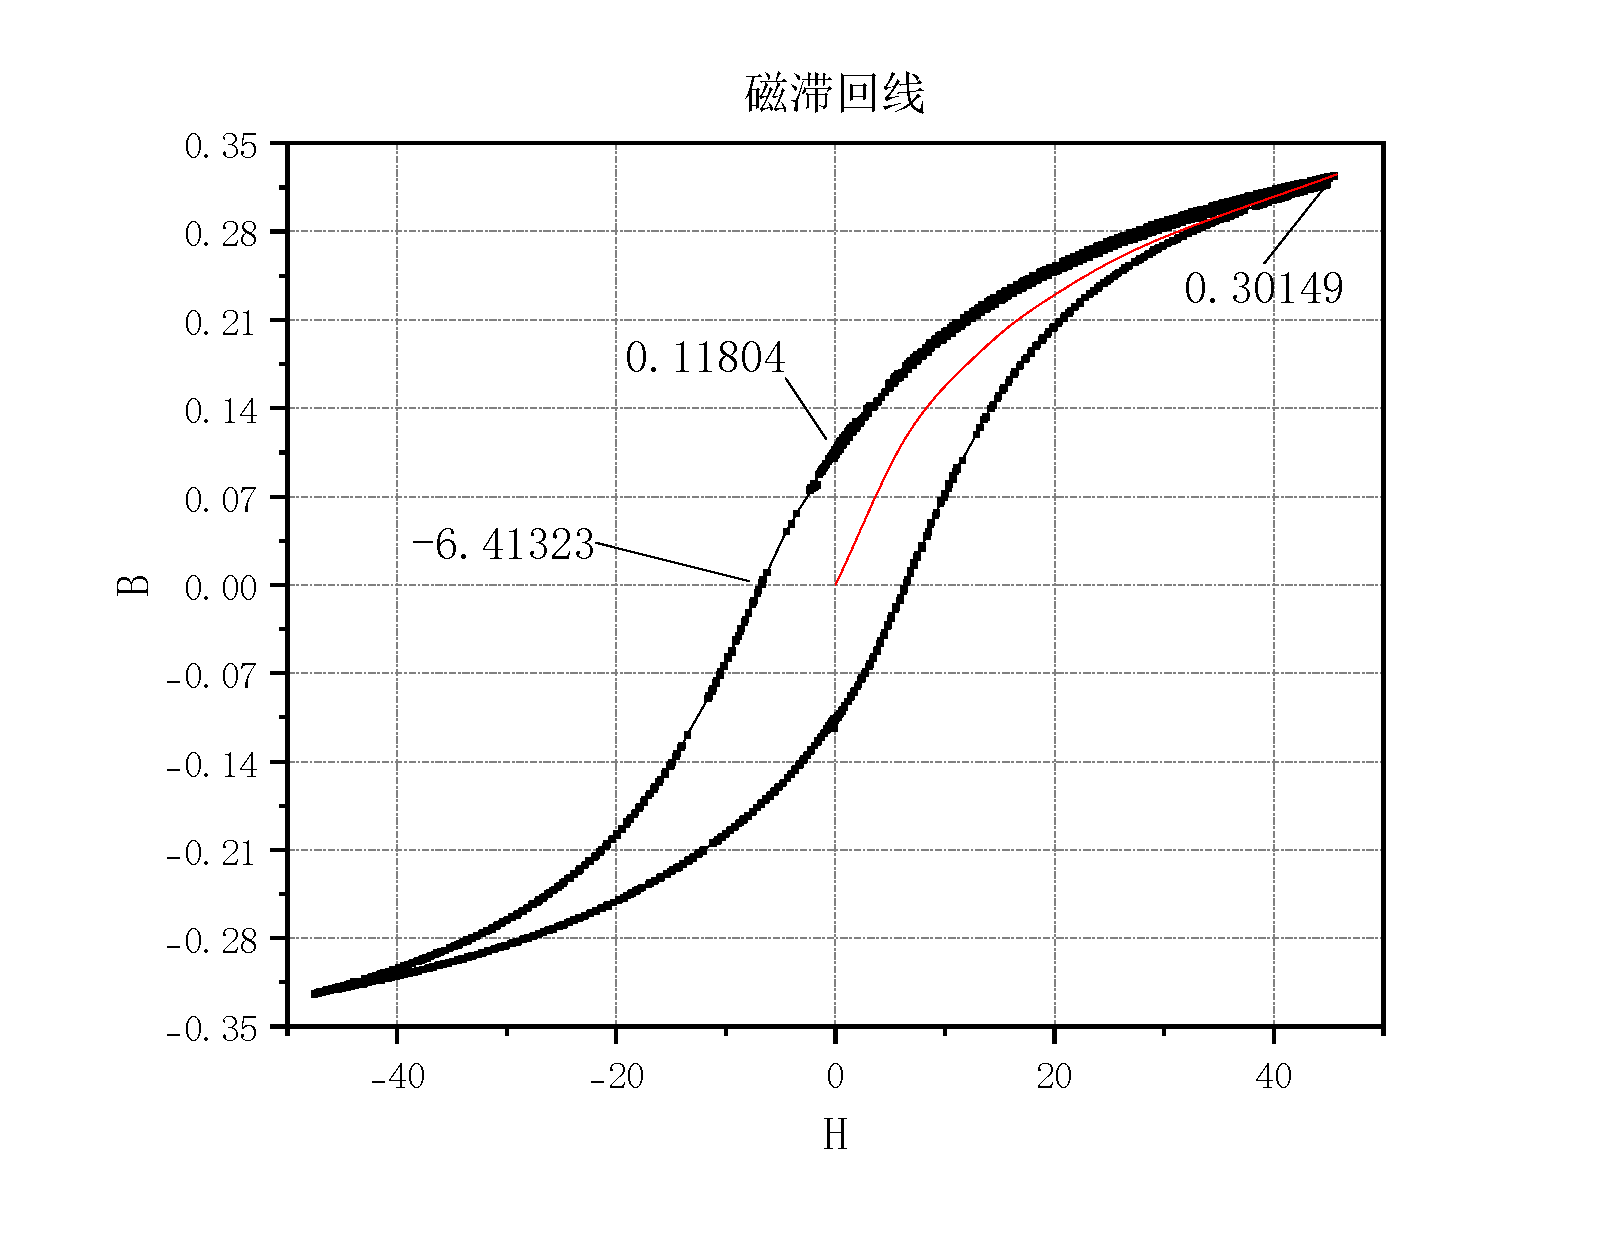
\includegraphics[width=0.6\textwidth]{fig3.pdf}
        \caption{0.8A磁滞回线}\label{fig:2b}
    \end{figure}
    \begin{figure}[!ht]
        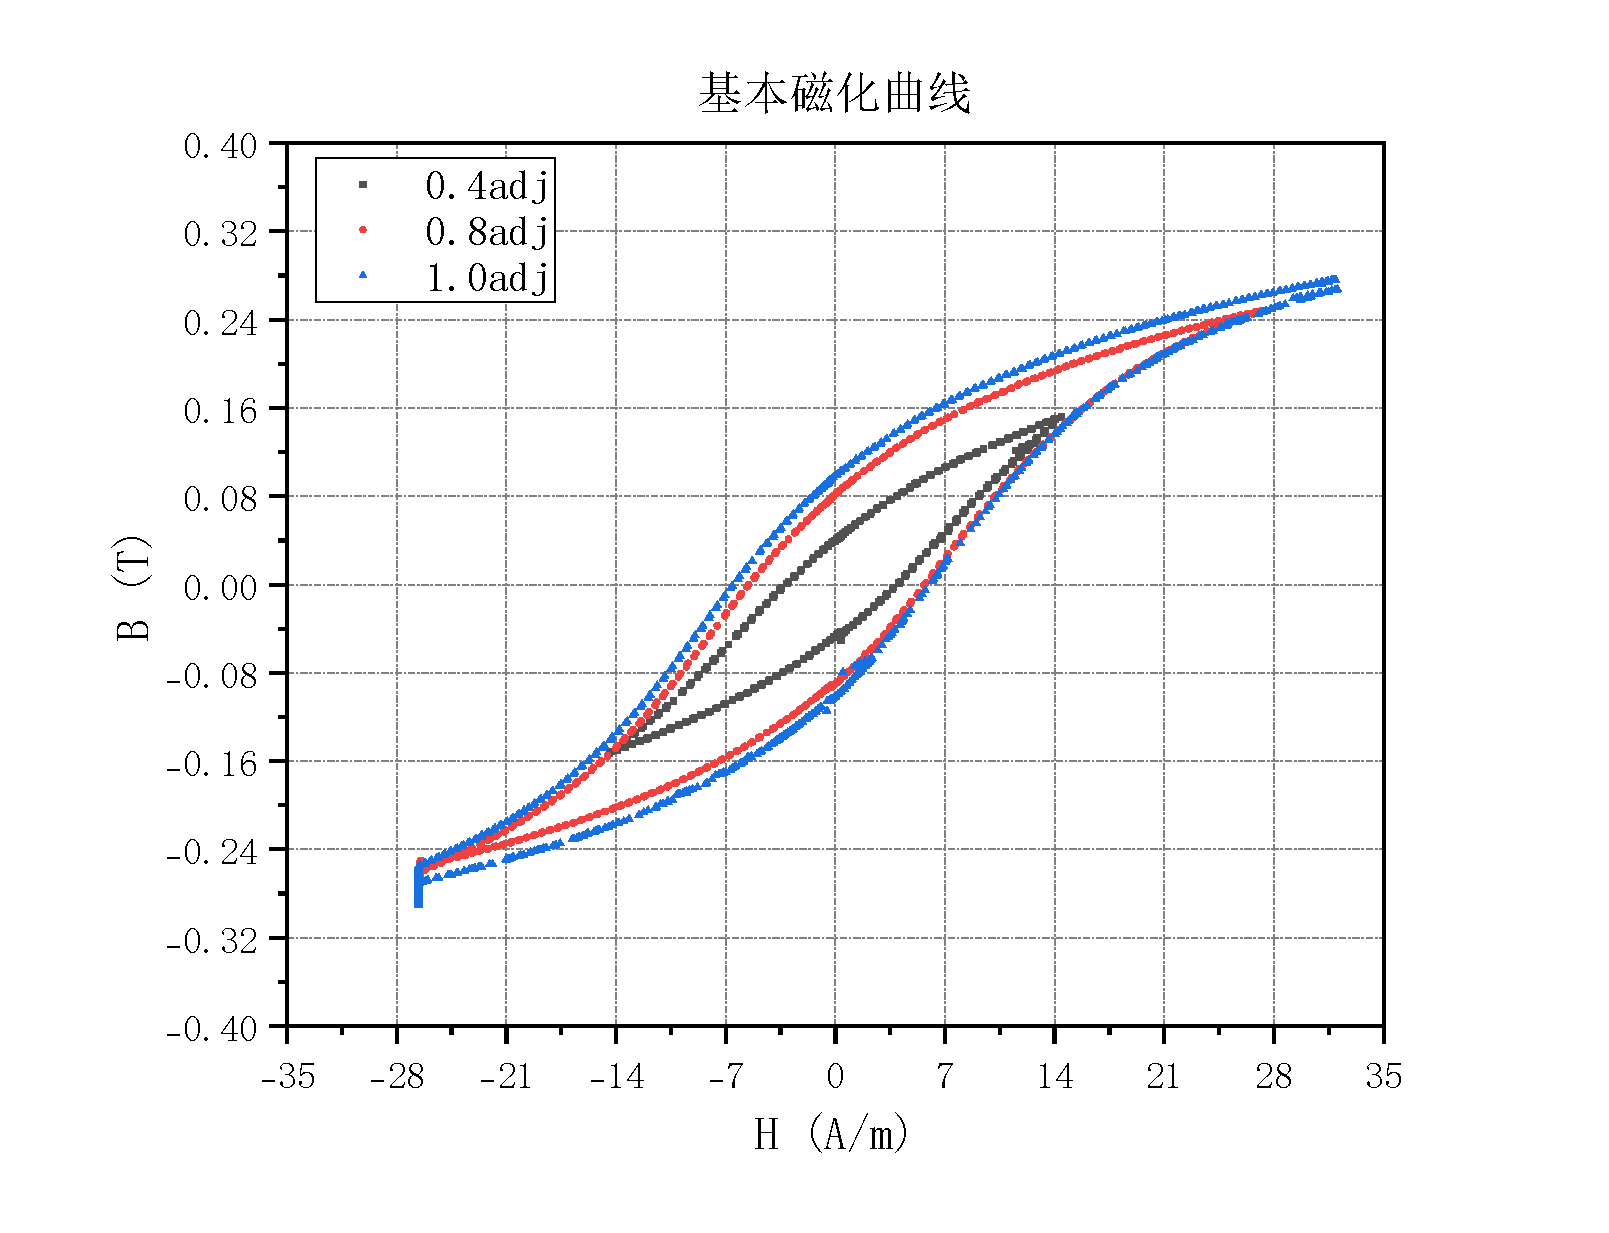
\includegraphics[width=0.6\textwidth]{fig4.pdf}
        \caption{基本磁化曲线}\label{fig:2c}
    \end{figure}
    \begin{figure}[!ht]
        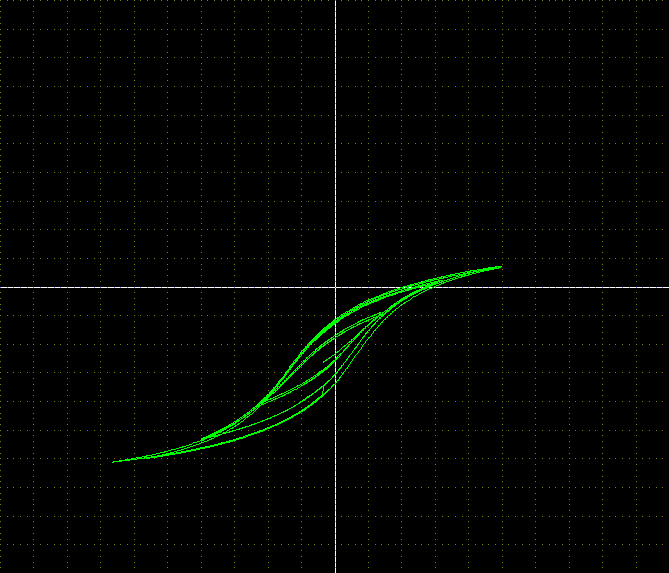
\includegraphics[width=0.4\textwidth]{fig5.png}
        \caption{软件原始输出}\label{fig:2d}
    \end{figure}
    \newpage
\section{结果分析}
    \subsection{图像分析}
        首先,由 \fgref{fig:2b} 可以得到在 \SI{0.8}{\A} 的磁化电流下,饱和磁感强度 $B_s= \SI{0.301}{\tesla}$,剩余磁感强度 $B_r= \SI{0.118}{\tesla}$,矫顽力 $H_c= \SI{-6.413}{\A\per\m}$。\par
        其次,在 \fgref{fig:2c} 中可以观察到在左下段出现了垂直向下的直线部分,这是因为 $U_x$ 超过了量程导致的,这种图形不可用于求饱和磁感强度,剩余磁感强度和矫顽力,因为其无法精确进行居中;此外,还能看到右上段并没有正确合拢,这很可能是由于“平衡”调节始终无法让电压表上的数字完全不变,随着测量进行,偏差将会不断积累。\par
        好在 \fgref{fig:2c} 最后重叠的结果与理论基本吻合,证明此次实验测得的结果基本无误。
    \subsection{误差分析}
        本次实验主要的误差来源有:
        \begin{itemize}
            \item 系统误差
                \begin{itemize}
                    \item 实验当天的温度、湿度对样品电磁性能的影响
                    \item 仪器本身精度的影响
                    \item 待测样品长久放置,很有可能会氧化或发生别的反应,改变性能
                \end{itemize}
            \item 偶然误差
                \begin{itemize}
                    \item 读电流值采用肉眼估测的方式,很容易导致电流过大或正负电流不相等,导致图像不对称
                    \item 在磁滞回线上取点时,往往数据点不能正好落在坐标轴上,只能以偏离后的值代替实际值计算
                \end{itemize}
        \end{itemize}
        可以通过:换用数字电流表、提高记录软件采样率、对样品进行恒温恒湿保管等方式来提高实验精度。
\section{思考题}
    \begin{enumerate}
        \item 测量初始磁化曲线时,为何没有出现 $B—H$ 的饱和区?\par
            这是因为此时磁化电流并不够大,大到几乎全部磁畴都已经转向外磁场方向。实验通常采用的是较小的磁场强度范围和较低的频率,以避免对样品造成不可逆的磁化,并且某些磁性材料可能具有较高的矫顽力,即需要较大的磁场才能使其磁化方向发生反转。本次实验所使用的最大电流都没有达到饱和状态,所以初始磁化曲线的电流明显不足以使材料磁化强度达到饱和状态。若要使初始磁化曲线出现 B-H 饱和区,可以通过增加线圈的匝数或者增大电流的强度,进而增大磁场强度,达到饱和。
        \item 实验中为何多次强调要单调地改变电流?否则会出现什么样的结果?\par
            在清除剩磁和测量磁滞回线这两个步骤中,我们就已经很清楚单调地改变电流,主要是为了避免出现磁滞效应,如果在实验中电流不是单调地改变,可能会由于磁滞效应而导致磁滞环的形成,这将会严重影响最后的图像。
        \item 根据从初始磁化曲线上求出的 B 和 H,能否绘出磁导率 μ 与 H 关系的曲线?\par
            能,如图:
            \begin{figure}[!ht]
                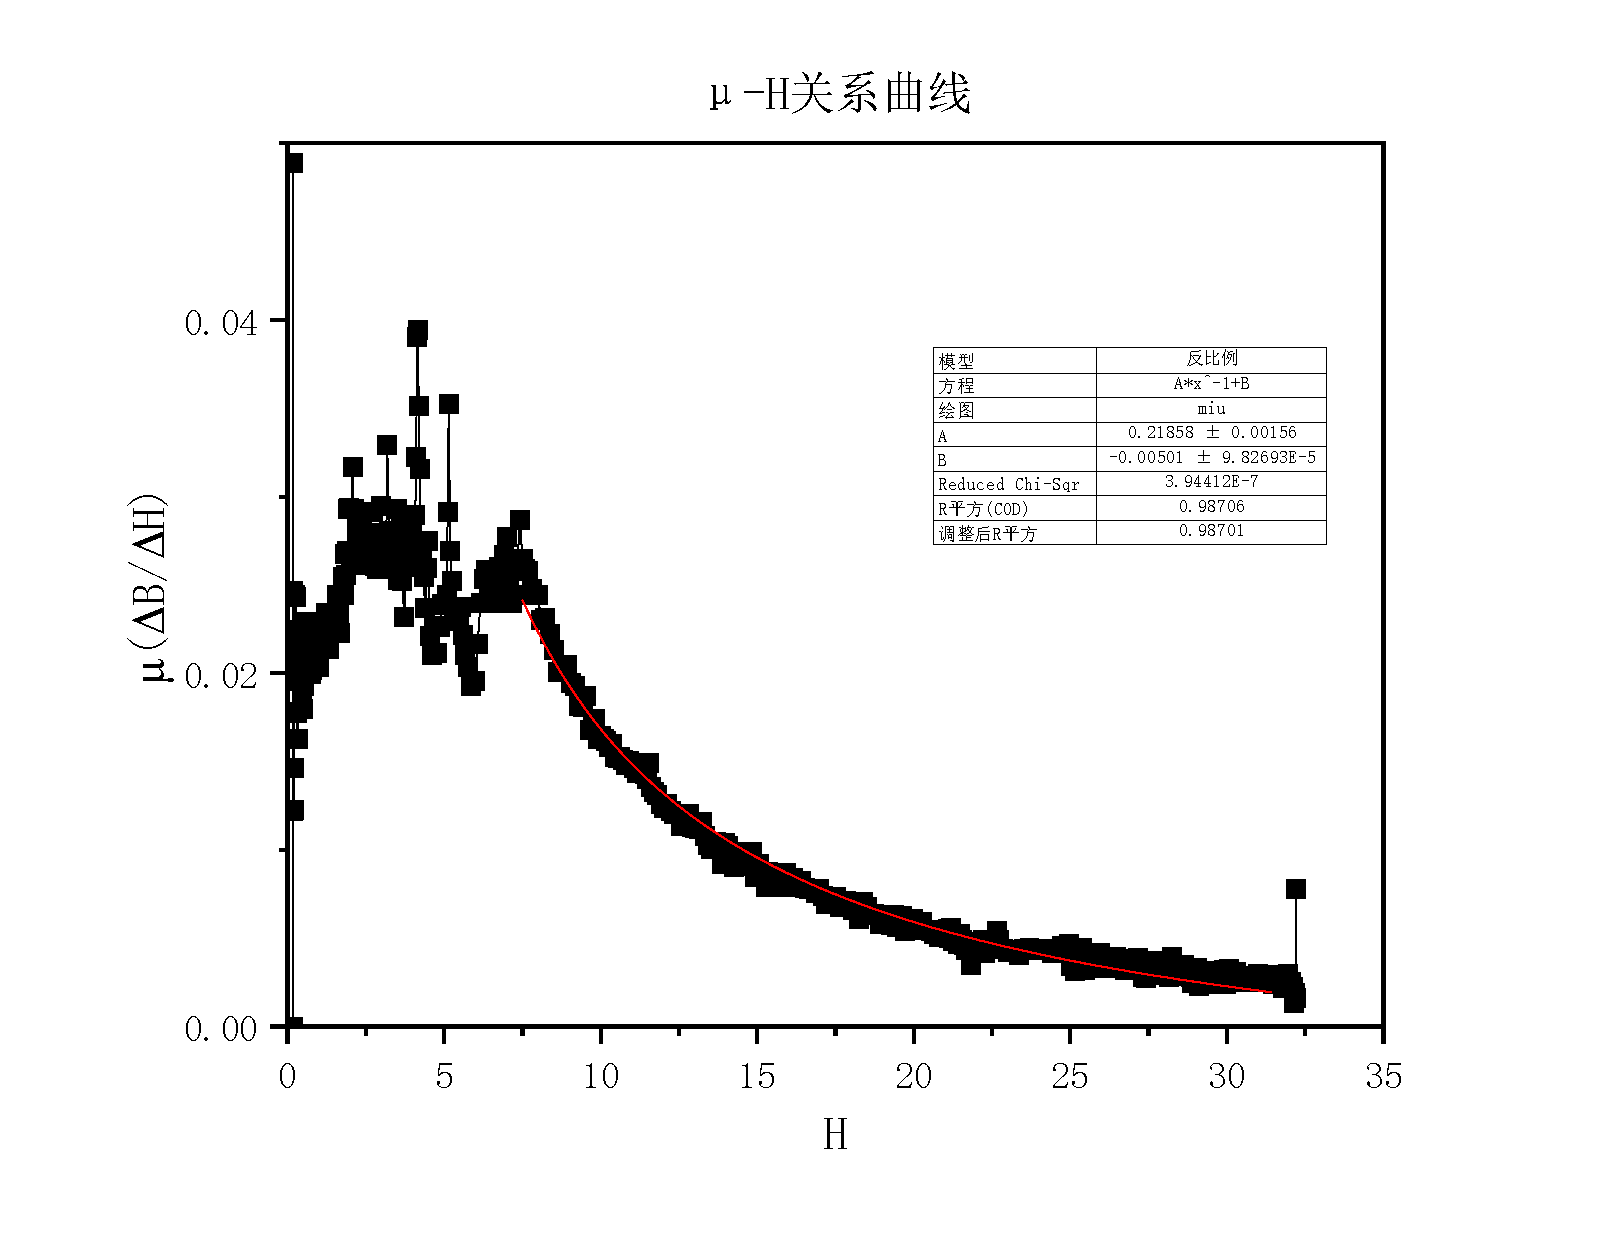
\includegraphics[width=0.8\textwidth]{fig6.pdf}
            \end{figure}
    \end{enumerate}
\part{交流磁化率}
\setcounter{section}{0}
\section{实验目的}
    \begin{itemize}
        \item 理解磁化率的基本概念并了解物质磁性的分类 
        \item 观察铁磁性转变及转变温度(居里温度)
        \item 测量不同铁磁样品的交流磁化率随温度的变化曲线
        \item 掌握测量不同铁磁样品的交流磁化率
    \end{itemize}
\section{实验原理}
    在给定的外界条件(T为常数)下,若材料各向异性,且 M//H,则磁化强度 M 和磁化率 $\chi$ 的关系为 $M=\chi H$ 。它的大小反映了物质磁化的难易程度,可正、可负,决定于材料的不同磁性类别。磁化率有三种表示形式, $\chi_V$ 表示单位体积(每 \unit{\cm^3})的磁化率,$\chi_A$表示每摩尔的磁化率,$\chi_g$表示单位质量(每 g)的磁化率,它们之间的关系为:
    \begin{equation}
        \chi_{A}=\chi_{V}V=\chi_{g}A=\frac{\chi_{A}A}{\delta}
    \end{equation}
    式中,A 为原子量,V 为每摩尔的体积,$\delta$ 为比重。磁体根据物质的磁化率大小和符号大致分为:抗磁性、顺磁性、反铁磁性、铁磁性和亚铁磁性。在外磁场作用下,抗磁性材料产生与其方向相反的磁矩,顺磁性材料产生方向相同的微弱磁性,遵循居里定律或居里-外斯定律。反铁磁性材料在一定温度下表现出与顺磁性相似的磁性,但在临界温度以上其磁化率降低并趋于定值,称为奈耳温度。铁磁性材料在小磁场下能被磁化到饱和,具有非线性的磁化强度和磁场关系,并在磁化过程中出现磁滞现象,其磁性随温度变化,居里温度是其特征参数。亚铁磁性材料与铁磁性相似,但磁化率较低,内部磁结构与反铁磁性相同。\par
    磁性物质具有自发性的磁偶极矩,在外加磁场下,物质中的磁偶极方向会因外界磁场作用而倾向沿着外加磁场方向。而当外加磁场是交变磁场且交流频率不太高时(一般在微波频率以下),磁偶极的方向可随着此外加交变磁场,做来回周期性振荡,此即交流磁化率的物理原因,交流磁化率 $\chi$ 可表示为:
    \begin{equation}
        \chi(\omega)=\chi’(\omega)+i\chi’’(\omega)
    \end{equation}\par
    交流磁化率测量方法主要有两类:一是交流互感电桥,如哈特森电桥。二是自感法,即测量样品在线圈中引起的电感变化。本实验采用自感法。
\section{实验仪器}
    锁相放大器、锁相波形发生器和加热炉、待测样品、计算机等
\section{实验过程}
    \begin{enumerate}
        \item 连接设备并启动软件
        \item 测量系统偏置
        \item 加热样品
        \item 调整本底电压
        \item 控制升温速率,测量降温
        \item 数据处理
    \end{enumerate}
\section{数据处理}
    见最后图:\par
    \begin{figure}[!ht]
        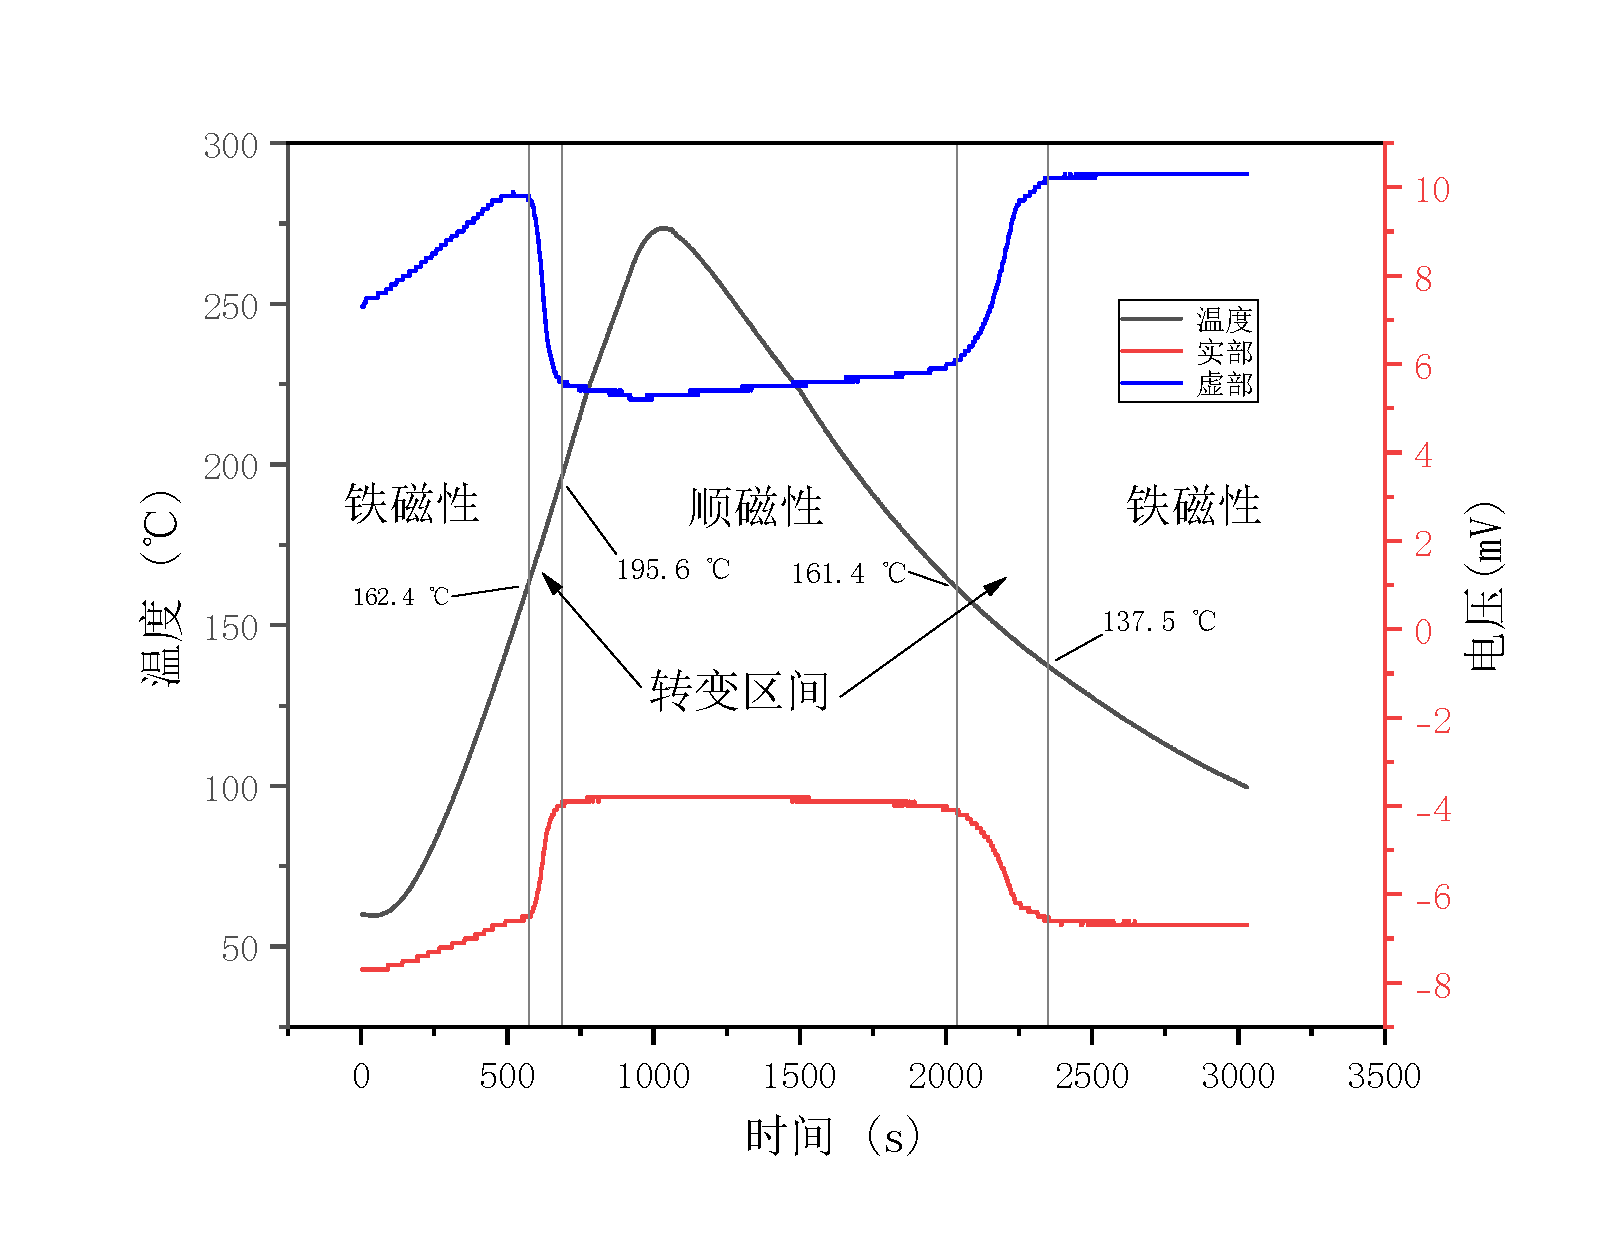
\includegraphics[width=0.7\textwidth]{fig7.pdf}
        \caption{温度、实部电压、虚部电压随时间变化曲线}\label{fig:7}
    \end{figure}\par
    \begin{figure}[!ht]
        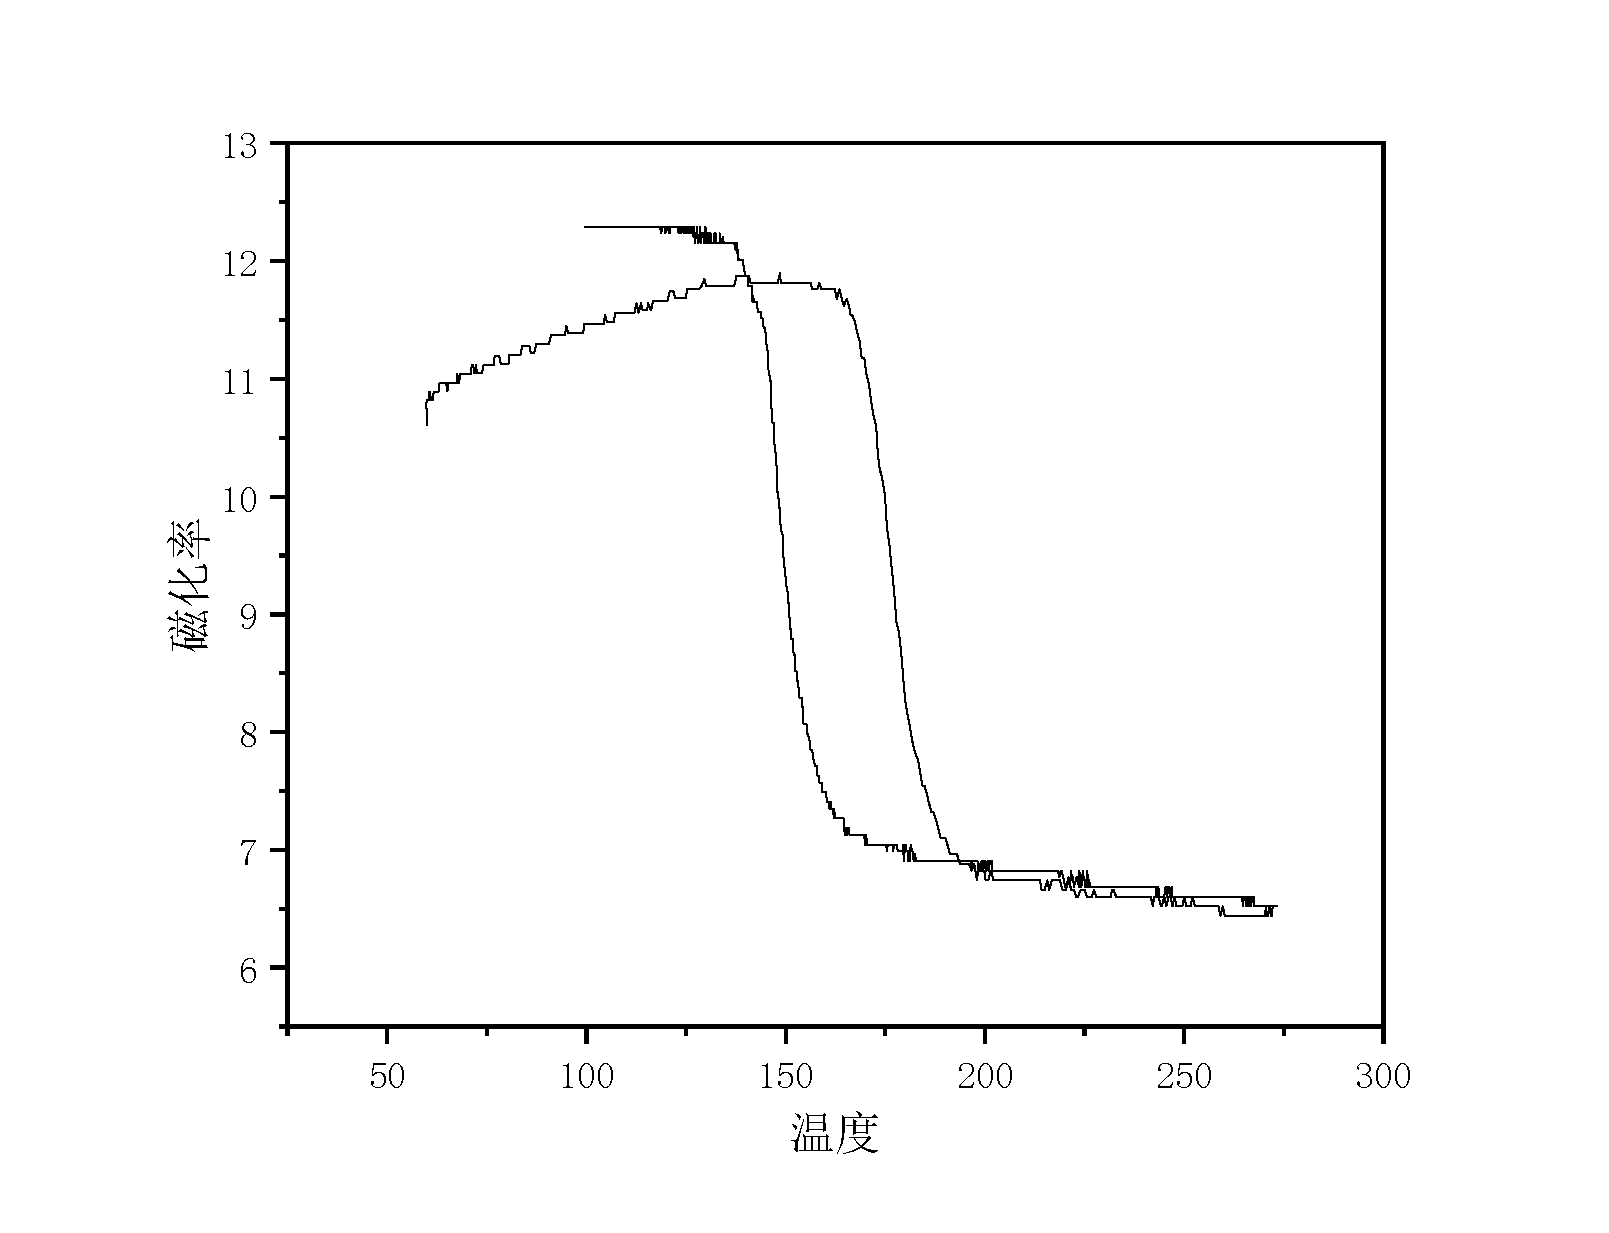
\includegraphics[width=0.7\textwidth]{fig8.pdf}
        \caption{磁化率*随温度变化曲线}\label{fig:8}
    \end{figure}\par
    \begin{figure}[!ht]
        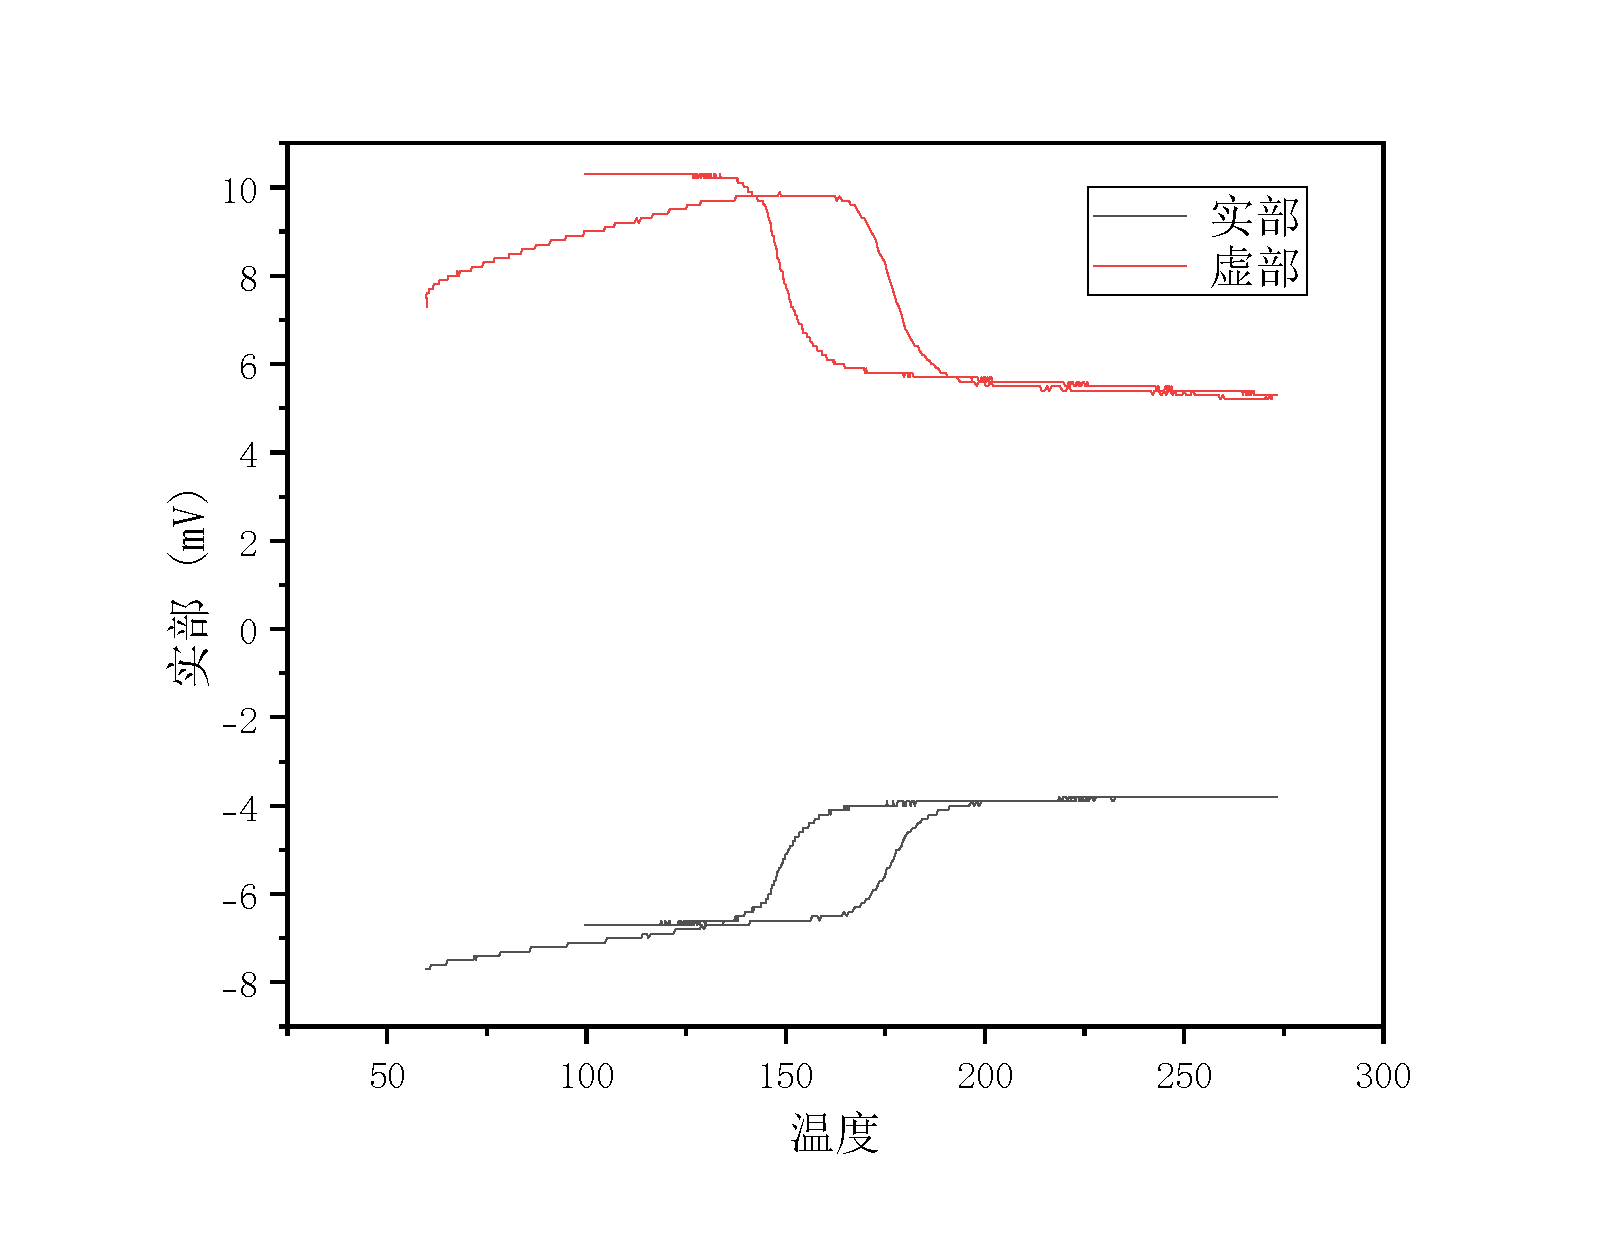
\includegraphics[width=0.7\textwidth]{fig9.pdf}
        \caption{实部电压、虚部电压随温度变化曲线}\label{fig:9}
    \end{figure}\par
\section{误差分析}
    本次实验主要的误差来源有:
    \begin{itemize}
        \item 系统误差
            \begin{itemize}
                \item 实验当天的温度、湿度、外电磁场对样品电磁性能的影响
                \item 仪器本身测量精度的影响
            \end{itemize}
        \item 偶然误差
            \begin{itemize}
                \item 在时间-电压线上取点时,拐点并不能准确判断,只能取得接近值代替实际值计算
            \end{itemize}
    \end{itemize}
    可以通过:提高记录软件采样率来提高实验精度。
\end{document}